\documentclass[border=10pt]{standalone}
\usepackage[svgnames]{xcolor}
\usepackage{amsmath}
\usepackage{pgfplots}
\pgfplotsset{compat=newest}
\usepackage[sfdefault]{FiraSans}
\usepackage{FiraMono}
\renewcommand*\familydefault{\sfdefault}
\begin{document}
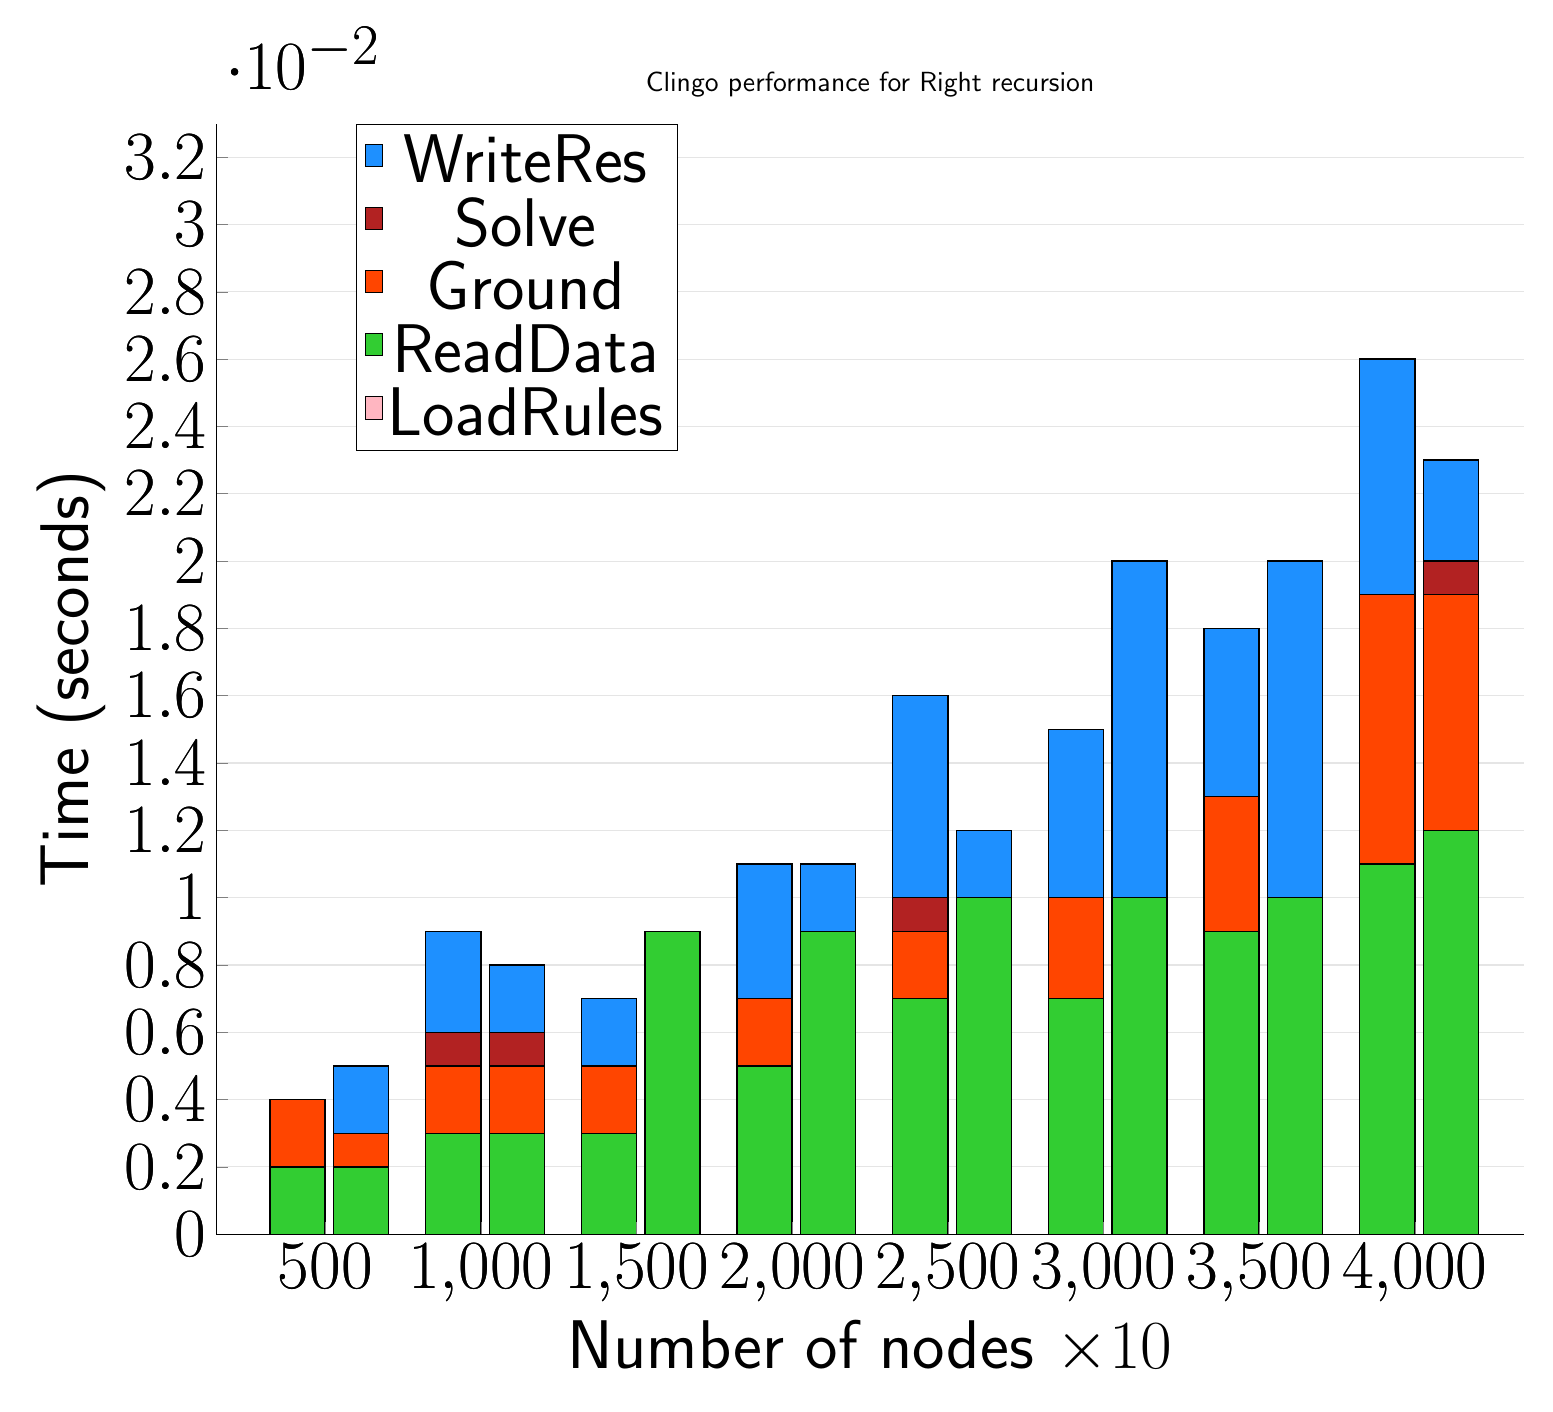
\begin{tikzpicture}
	\begin{axis}[
			ybar stacked,
			title={Clingo performance for Right recursion},
			bar shift=-10pt,
			width=1.5\textwidth,
			bar width=0.7cm,
			ymajorgrids, tick align=inside,
			major grid style={draw=gray!20},
			xtick=data,
			ymin=0, ymax=0.03299998760223389,
			axis x line*=bottom,
			axis y line*=left,
			enlarge x limits=0.1,
			legend style={
					at={(0.23, 1)},
					anchor=north,
					legend columns=1,
					font=\Huge,
				},
			ylabel={Time (seconds)},
			xlabel={Number of nodes $\times 10$},
			label style={font=\Huge},
			tick label style={font=\Huge},
		]
		\addlegendimage{fill=DodgerBlue, draw=black, line width=0.2pt}
		\addlegendentry{WriteRes}
		\addlegendimage{fill=FireBrick, draw=black, line width=0.2pt}
		\addlegendentry{Solve}
		\addlegendimage{fill=OrangeRed, draw=black, line width=0.2pt}
		\addlegendentry{Ground}
		\addlegendimage{fill=LimeGreen, draw=black, line width=0.2pt}
		\addlegendentry{ReadData}
		\addlegendimage{fill=LightPink, draw=black, line width=0.2pt}
		\addlegendentry{LoadRules}
		\addplot +[fill=LightPink, draw=black, line width=0.5pt] coordinates {
				(500, 0.0)
				(1000, 0.0)
				(1500, 0.0)
				(2000, 0.0)
				(2500, 0.0)
				(3000, 0.0)
				(3500, 0.0)
				(4000, 0.0)
			};
		\addplot +[fill=LimeGreen, draw=black, line width=0.5pt] coordinates {
				(500, 0.0019999980926513673)
				(1000, 0.0029999971389770507)
				(1500, 0.0029999971389770507)
				(2000, 0.004999995231628418)
				(2500, 0.006999993324279785)
				(3000, 0.006999993324279785)
				(3500, 0.008999991416931152)
				(4000, 0.01099998950958252)
			};
		\addplot +[fill=OrangeRed, draw=black, line width=0.5pt] coordinates {
				(500, 0.0019999980926513673)
				(1000, 0.0019999980926513673)
				(1500, 0.0019999980926513673)
				(2000, 0.0019999980926513673)
				(2500, 0.0019999980926513673)
				(3000, 0.0029999971389770507)
				(3500, 0.0039999961853027345)
				(4000, 0.008000016212463379)
			};
		\addplot +[fill=FireBrick, draw=black, line width=0.5pt] coordinates {
				(500, 0.0)
				(1000, 0.0009999990463256836)
				(1500, 0.0)
				(2000, 0.0)
				(2500, 0.0009999990463256836)
				(3000, 0.0)
				(3500, 0.0)
				(4000, 0.0)
			};
		\addplot +[fill=DodgerBlue, draw=black, line width=0.5pt] coordinates {
				(500, 0.0)
				(1000, 0.0029999971389770507)
				(1500, 0.0019999980926513673)
				(2000, 0.004000020027160644)
				(2500, 0.006000018119812012)
				(3000, 0.004999995231628418)
				(3500, 0.004999995231628418)
				(4000, 0.0070000171661376955)
			};
	\end{axis}
	\begin{axis}[
			ybar stacked,
			bar shift=13pt,
			width=1.5\textwidth,
			bar width=0.7cm,
			ymajorgrids, tick align=inside,
			major grid style={draw=none},
			xtick=data,
			ymin=0, ymax=0.03299998760223389,
			axis x line*=none,
			axis y line*=none,
			enlarge x limits=0.1,
			label style={font=\Huge},
			tick label style={font=\Huge},
		]
		\addplot +[fill=LightPink, draw=black, line width=0.5pt] coordinates {
				(500, 0.0)
				(1000, 0.0)
				(1500, 0.0)
				(2000, 0.0)
				(2500, 0.0)
				(3000, 0.0)
				(3500, 0.0)
				(4000, 0.0)
			};
		\addplot +[fill=LimeGreen, draw=black, line width=0.5pt] coordinates {
				(500, 0.0019999999999999996)
				(1000, 0.0029999999999999996)
				(1500, 0.008999999999999998)
				(2000, 0.008999999999999998)
				(2500, 0.009999999999999997)
				(3000, 0.009999999999999997)
				(3500, 0.009999999999999997)
				(4000, 0.011999999999999997)
			};
		\addplot +[fill=OrangeRed, draw=black, line width=0.5pt] coordinates {
				(500, 0.0009999999999999998)
				(1000, 0.0019999999999999996)
				(1500, 0.0)
				(2000, 0.0)
				(2500, 0.0)
				(3000, 0.0)
				(3500, 0.0)
				(4000, 0.007000000000000001)
			};
		\addplot +[fill=FireBrick, draw=black, line width=0.5pt] coordinates {
				(500, 0.0)
				(1000, 0.0009999999999999998)
				(1500, 0.0)
				(2000, 0.0)
				(2500, 0.0)
				(3000, 0.0)
				(3500, 0.0)
				(4000, 0.0010000000000000002)
			};
		\addplot +[fill=DodgerBlue, draw=black, line width=0.5pt] coordinates {
				(500, 0.0019999999999999996)
				(1000, 0.002)
				(1500, 0.0)
				(2000, 0.0020000000000000005)
				(2500, 0.0020000000000000005)
				(3000, 0.010000000000000004)
				(3500, 0.010000000000000004)
				(4000, 0.0030000000000000005)
			};
	\end{axis}
\end{tikzpicture}

\end{document}
